
\documentclass[12pt,a4paper]{article}
\usepackage{graphicx}
\usepackage{amsmath}
\usepackage{amssymb}
\usepackage{listings}
\usepackage{geometry}

\geometry{margin=1in}
\begin{document}
\noindent

\begin{minipage}{0.6\textwidth}

\includegraphics[width=0.75\textwidth]{IIITB-COMET-Logo.png}
\end{minipage}
\begin{minipage}{0.38\textwidth}
\begin{center}
\textbf{DARSI VAMSI}
\newline
\textbf{COMET FWC 071}
\end{center}
\end{minipage}
\newline
\newline
\begin{center}
    {\LARGE\textbf{Implementation of the Boolean Function}}\\[0.3cm]
    {\LARGE\textbf{$Y=AB+CD$ Using Raspberry Pi Pico 2 W}}
    \\
    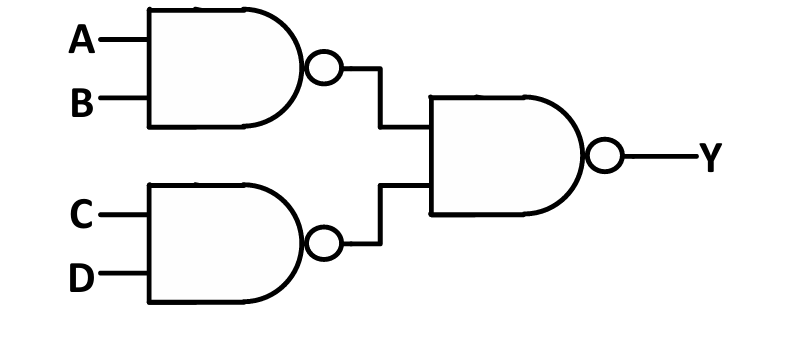
\includegraphics[width=0.75\textwidth]{figure.png}
\end{center}


\section{Problem Analysis}

The given logic circuit consists of three NAND gates.

The output of the first NAND gate is

$$
X_1=(AB)'
$$

The output of the second NAND gate is

$$
X_2=(CD)'
$$

The final output is

$$
Y=(X_1X_2)'
$$

Substituting the values of $X_1$ and $X_2$,

$$
Y=((AB)'(CD)')'
$$

Applying De Morgan's theorem,

$$
Y=((AB)')'+((CD)')'
$$

Therefore,

$$
\boxed{Y=AB+CD}
$$

The output becomes logic '1' whenever:

\begin{itemize}
    \item $A=1$ and $B=1$, or
    \item $C=1$ and $D=1$.
\end{itemize}

Otherwise, the output remains logic '0'.
\section{Hardware Requirements}

\begin{itemize}
    \item Raspberry Pi Pico 2 W Development Board
    \item USB Type-C Cable
    \item Personal Computer or Laptop
    \item LED
    \item 220 $\Omega$ Resistor
    \item Breadboard and Connecting Wires
\end{itemize}
\section{Pin Connections with Raspberry Pi Pico 2 W}

\begin{center}
\begin{tabular}{|c|c|}
\hline
\textbf{Component} & \textbf{Raspberry Pi Pico 2 W Pin} \\
\hline
LED Anode (+) & GP1 \\
\hline
LED Cathode (-) & GND through 220 $\Omega$ resistor \\
\hline
\end{tabular}
\end{center}

No external switches are used because the input combinations are generated within the program itself.
```latex
\section{Hardware Setup and Accessing Raspberry Pi Pico 2 W Using Arduino IDE}

The Raspberry Pi Pico 2 W is programmed using the Arduino IDE by installing the necessary board support packages and configuring the development environment. The detailed procedure is as follows.



\subsection{Installing Arduino IDE}

\begin{enumerate}
    \item Download and install the latest version of Arduino IDE from the official Arduino website.
    \item Open the Arduino IDE after installation.
\end{enumerate}

\subsection{Installing Raspberry Pi Pico 2 W Board Package}

\begin{enumerate}
    \item Open Arduino IDE.
    \item Navigate to
    \[
    \text{File} \rightarrow \text{Preferences}
    \]
    
    \item In the ``Additional Boards Manager URLs'' field, add the following URL:
    
\begin{verbatim}
https://github.com/earlephilhower/arduino-pico/releases/download/global/package_rp2040_index.json
\end{verbatim}

    \item Click ``OK''.
    
    \item Navigate to
    \[
    \text{Tools} \rightarrow \text{Board} \rightarrow \text{Boards Manager}
    \]

    \item Search for ``Raspberry Pi Pico/RP2040''.

    \item Install the package developed by Earle F. Philhower.
\end{enumerate}

\subsection{Connecting the Raspberry Pi Pico 2 W}

\begin{enumerate}
    \item Connect the Raspberry Pi Pico 2 W to the computer using a USB Type-C cable.
    
    \item If the board is not detected automatically:
    \begin{enumerate}
        \item Press and hold the \textbf{BOOTSEL} button.
        \item Connect the USB cable while holding the button.
        \item Release the button after the board appears as a removable drive.
    \end{enumerate}
\end{enumerate}

\subsection{Selecting the Board and Port}

\begin{enumerate}
    \item Navigate to
    \[
    \text{Tools} \rightarrow \text{Board}
    \]

    \item Select
    \[
    \text{Raspberry Pi Pico 2 W}
    \]

    \item Navigate to
    \[
    \text{Tools} \rightarrow \text{Port}
    \]

    \item Select the corresponding COM port of the Raspberry Pi Pico 2 W.
\end{enumerate}

\subsection{Uploading the Program}

\begin{enumerate}
    \item Write or paste the Arduino program into the Arduino IDE.
    \item Click the \textbf{Verify} button to compile the code.
    \item Click the \textbf{Upload} button.
    \item Wait until the message

Done Uploading\\
appears in the output window.
\end{enumerate}


After successful uploading of the program, the Raspberry Pi Pico 2 W executes the Boolean expression

$$
Y = AB + CD
$$

for all possible input combinations and displays the output through the LED connected to GP1.

\section{Implementing Algorithm in Raspberry Pi Pico 2W}

\subsection{Algorithm}

\begin{enumerate}
    \item Start the program written in the codes sections .
    \item Configure GP1 as OUTPUT.
    \item Initialize variables $A$, $B$, $C$, and $D$.
    \item Generate all possible combinations of inputs using nested loops.
    \item Compute the output

    $$
    Y=(A \& B)|(C \& D)
    $$

    \item If $Y=1$, turn ON the LED connected to GP1.
    \item If $Y=0$, turn OFF the LED.
    \item Wait for one second.
    \item Repeat for all sixteen input combinations continuously.
\end{enumerate}


\section{Result}

The Boolean expression

$$
\boxed{Y=AB+CD}
$$

was successfully implemented on the Raspberry Pi Pico 2 W using Arduino IDE. The LED connected to GP1 turned ON whenever the output of the logic function was '1' and turned OFF whenever the output was '0'. The program successfully verified all sixteen possible combinations of the four input variables.
\begin{center}
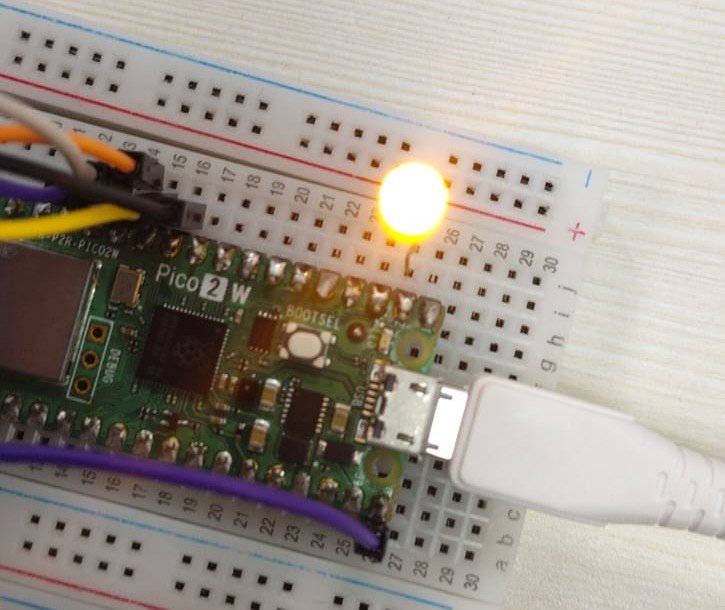
\includegraphics[width=0.65\textwidth]{Led_gate_pico2w.jpeg}
\end{center}
\end{document}

